%\immediate\write18{tex ../tikzmark.dtx}
\documentclass[a4paper]{article}
\usepackage{amsmath}
\usepackage{tikz}
\usepackage{lipsum}
\usepackage{listings}
\usetikzlibrary{
  arrows.meta,
  tikzmark,
  fit,
  shadows
}
\usetikzmarklibrary{%
  highlighting,
  ams,
  listings
}

\tikzset{>=Latex}

\title{TikZmark Tests}
\author{Andrew Stacey}
\date{\today}

\begin{document}

\maketitle

\section{Basic Tests}

There is a tikzmark here\tikzmark{a} and a tikzmark here\tikzmark{b}.
Let's join them together.
\tikz[remember picture, overlay] {\draw[<->] (pic cs:a) to[out=90,in=90] (pic cs:b);}

There is a tikzmark node \tikzmarknode{c}{here} and a tikzmark node \tikzmarknode{d}{here}.
Let's join them together.
\tikz[remember picture, overlay] {\draw[<->,red] (pic cs:c) to[out=-90,in=-90] (pic cs:d); \draw[<->,blue] (c) to[out=90,in=90] (d);}

Here is a tikzmark inside a tikz picture \tikz[remember picture] { \draw (0,0) rectangle (1,1); \tikzmark{f}{(.5,.5)}}.
Now let's draw using it.\tikz[remember picture, overlay] {\draw[green,<-] (pic cs:f) -- +(0,1);}

\section{Subnodes in Maths}

\begin{itemize}
\item Display style
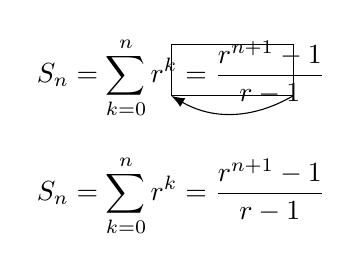
\begin{tikzpicture}[remember picture,baseline=-1]
\node {\(\displaystyle S_n = \sum_{k=0}^n r^k = \frac{r^{n+1} - 1}{r-1} \)};
\node at (0,-1.5) {\(\displaystyle S_n = \subnode{da}{\sum_{k=0}^n r^k} = \frac{r^{n+1} - 1}{r-1} \)};
\draw[->] (da.south east) to[bend left] (da.south west);
\node[fit=(da),draw,inner sep=0pt,node contents={}];
\end{tikzpicture}

\item Text style
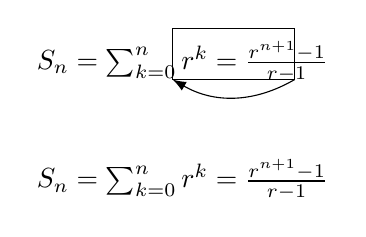
\begin{tikzpicture}[remember picture,baseline=-1]
\node {\(S_n = \sum_{k=0}^n r^k = \frac{r^{n+1} - 1}{r-1} \)};
\node at (0,-1.5) {\(S_n = \subnode{ta}{\sum_{k=0}^n r^k} = \frac{r^{n+1} - 1}{r-1} \)};
\draw[->] (ta.south east) to[bend left] (ta.south west);
\node[fit=(ta),draw,inner sep=0pt,node contents={}];
\end{tikzpicture}

\item Script style
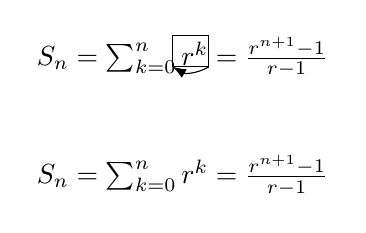
\begin{tikzpicture}[remember picture,baseline=-1]
\node {\(S_n = \sum_{k=0}^n r^k = \frac{r^{n+1} - 1}{r-1} \)};
\node at (0,-1.5) {\(S_n = \sum_{k=0}^{\subnode{sa}{n}} r^k = \frac{r^{n+1} - 1}{r-1} \)};
\draw[->] (sa.south east) to[bend left] (sa.south west);
\node[fit=(sa),draw,inner sep=0pt,node contents={}];
\end{tikzpicture}

\item Script script style
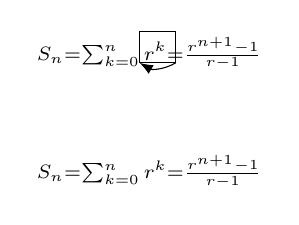
\begin{tikzpicture}[remember picture,baseline=-1]
\node {\(\scriptstyle S_n = \sum_{k=0}^n r^k = \frac{r^{n+1} - 1}{r-1} \)};
\node at (0,-1.5) {\(\scriptstyle S_n = \sum_{k=0}^{\subnode{ssa}{n}} r^k = \frac{r^{n+1} - 1}{r-1} \)};
\draw[->] (ssa.south east) to[bend left] (ssa.south west);
\node[fit=(ssa),draw,inner sep=0pt,node contents={}];
\end{tikzpicture}

\end{itemize}


\section{Testing transformations}

There's a tikzmark\tikzmark{l} here

\begin{tikzpicture}[remember picture, overlay]
\draw (0,0) -- (1,-1);
\draw[->] (0,0) to[bend left] (pic cs:l);
\end{tikzpicture}

\begin{tikzpicture}[remember picture, overlay, shift={(1cm,-1cm)}, scale=2]
\draw (0,0) -- (1,-1);
\draw[->] (0,0) to[bend left] (pic cs:l);
\end{tikzpicture}

\section{Testing inside tikzpicture}

\begin{tikzpicture}
\tikzmark{inside a}{(1,2)}
\draw[->] (0,0) -- (pic cs:inside a);
\fill[blue] (1,2) circle[radius=3pt];
\fill[green] (0,0) circle[radius=3pt];
\begin{scope}[shift={(2,1)},rotate=30,scale=.8]
\tikzmark{inside b}{(1,2)}
\fill[red] (1,2) circle[radius=3pt];
\fill[orange] (0,0) circle[radius=3pt];
\draw[->] (0,0) -- (pic cs:inside a);
\end{scope}
\draw[->] (0,0) -- (pic cs:inside b);
\end{tikzpicture}

\section{Testing Prefix/Suffix}

\begin{itemize}
\item Without suffix:
\tikzmark{bar}
\iftikzmark{bar}{
  TIKZMARK BAR IS AVAILABLE
}{
  TIKZMARK BAR IS NOT AVAILABLE
}


\item With suffix:
\tikzset{tikzmark suffix=-foo}%
\tikzmark{baz}
\iftikzmark{baz}{
  TIKZMARK BAZ IS AVAILABLE
}{
  TIKZMARK BAZ IS NOT AVAILABLE
}
\end{itemize}

\section{Inside a Box}

\newbox\mybox

We're about to create a box containing a pgfmark:
\savebox\mybox{\pgfmark{h}hello world}%
it has now been created.

\wd\mybox=0pt\relax
\ht\mybox=0pt\relax
\dp\mybox=0pt\relax

Now we used it: \unhbox\mybox\
it has been used

\vspace{2cm}

Let's point to the pgfmark in the box.
\tikz[remember picture,overlay] \draw[->] (0,0) to[bend right] (pic cs:h);

\section{Subnode tests}

Tests using subnode.

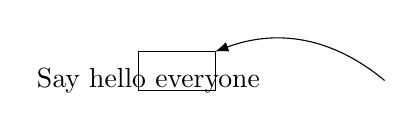
\begin{tikzpicture}[remember picture]
\node {Say \subnode{i}{hello} everyone};
\node[fit=(i),draw,inner sep=0pt] {};
\draw[->] (3,0) to[bend right] (i.north east);
\end{tikzpicture}


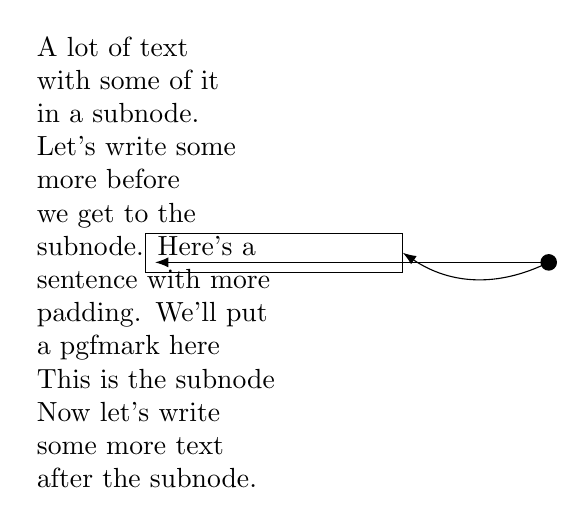
\begin{tikzpicture}[remember picture]
\node[text width=3cm] {A lot of text with some of it in a subnode.
Let's write some more before we get to the subnode.
Here's a sentence with more padding.
We'll put a pgfmark here\pgfmark{j}
\subnode{k}{This is the subnode}
Now let's write some more text after the subnode.
};
\fill (5,0) circle[radius=3pt] coordinate (src);
\draw[->] (src) to[bend left] (k.east);
\node[fit=(k),draw,inner sep=0pt] {};
\draw[->] (src) -- (pic cs:j);
\end{tikzpicture}



Testing box sizes:

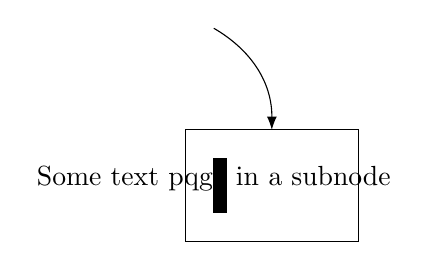
\begin{tikzpicture}[remember picture]
\node {Some \subnode[inner sep=10pt]{m}{text pqg\rule[-10pt]{5pt}{20pt}} in a subnode};
\draw[->] (0,2) to[bend left] (m.north);
\node[fit=(m),draw,inner sep=0pt] {};
\end{tikzpicture}

\newpage
\section{Listings Tests}

\tikzset{
  next page=below,
%  every highlighter/.style={rounded corners},
  line/.style={
    draw,
    rounded corners=3pt,
    -latex
  },
  balloon/.style={
    draw,
    fill=blue!20,
    opacity=0.4,
    inner sep=4pt,
    rounded corners=2pt
  },
  comment/.style={
    draw,
    fill=blue!70,
    text=white,
%    text width=3cm,
%    minimum height=1cm,
    rounded corners,
    drop shadow,
    align=left,
%    font=\scriptsize
  },
}

\newcommand\balloon[4]{%
  \pgfmathtruncatemacro\firstline{%
    #3-1
  }%
  \iftikzmark{line-#2-\firstline-start}{%
    \iftikzmark{line-#2-#3-first}{%
      \xdef\blines{({pic cs:line-#2-\firstline-start} -| {pic           cs:line-#2-#3-first})}%
    }{%
      \iftikzmark{line-#2-#3-start}{%
        \xdef\blines{({pic cs:line-#2-\firstline-start} -| {pic             cs:line-#2-#3-start})}%
      }{%
        \xdef\blines{(pic cs:line-#2-\firstline-start)}%
      }%
    }%
  }{%
    \xdef\blines{}%
  }%
  \foreach \k in {#3,...,#4} {%
    \iftikzmark{line-#2-\k-first}{%
      \xdef\blines{\blines (pic cs:line-#2-\k-first) }
    }{}
    \iftikzmark{line-#2-\k-end}{%
      \xdef\blines{\blines (pic cs:line-#2-\k-end) }
    }{}
  }%
  \ifx\blines\empty
  \else
  \edef\temp{\noexpand\tikz[remember picture,overlay]\noexpand\node[fit={\blines},balloon] (#1) {};}%
\temp
  \fi
}


\begin{lstlisting}[language=TeX,name=texcode,numbers=left,breakatwhitespace=true,breaklines=true]
\newcommand\balloon[4]{%
  \pgfmathtruncatemacro\firstline{%
    #3-1
  }%
  \iftikzmark{line-#2-\firstline-start}{%
    \iftikzmark{line-#2-#3-first}{%
      \xdef\blines{({pic cs:line-#2-\firstline-start} -| {pic           cs:line-#2-#3-first})}%
    }{%
      \iftikzmark{line-#2-#3-start}{%
        \xdef\blines{({pic cs:line-#2-\firstline-start} -| {pic             cs:line-#2-#3-start})}%
      }{%
        \xdef\blines{(pic cs:line-#2-\firstline-start)}%
      }%
    }%
  }{%
    \xdef\blines{}%
  }%
  \foreach \k in {#3,...,#4} {%
    \iftikzmark{line-#2-\k-first}{%
      \xdef\blines{\blines (pic cs:line-#2-\k-first) }
    }{}
    \iftikzmark{line-#2-\k-end}{%
      \xdef\blines{\blines (pic cs:line-#2-\k-end) }
    }{}
  }%
  \ifx\blines\empty
  \else
  \edef\temp{\noexpand\tikz[remember picture,overlay] \noexpand\node[fit={\blines},balloon] (#1) {};}%
\temp
  \fi
}
\end{lstlisting}

\begin{tikzpicture}[remember picture,overlay,>=Latex]
\draw[<-,ultra thick] (pic cs:line-texcode-1-end) +(1em,.7ex) -| +(2.5,1) node[above,comment,thin] {Command name};
\draw[<-,ultra thick] (pic cs:line-texcode-3-end) ++(1em,.7ex) -| +(5.8,1) node[above right,comment,thin] {Find previous line};
\draw[<-,ultra thick] (pic cs:line-texcode-5-end) ++(1em,.7ex) -| +(2.2,.5) node[above,comment,thin] {If previous line exists, add to the list};
\draw[<-,ultra thick] (pic cs:line-texcode-18-end) ++(1em,.7ex) -| +(2.2,.5) node[above,comment,thin] {Loop through rest of lines};
\draw[<-,ultra thick] (pic cs:line-texcode-28-end) ++(1em,.7ex) -| +(1,1.5) node[above,comment,thin] {Add a node covering all the lines};
\end{tikzpicture}

\newpage

\section{Tikzmarks on other pages}

\tikz[overlay,remember picture,ultra thick,red] \draw (pic cs:n) -- (pic cs:o);%
A\tikzmark{n} tikzmark

\lipsum[1-4]
\lipsum[4]
\lipsum*[4]
\tikzmark{o}%

\lipsum[1]
\tikz[overlay,remember picture,ultra thick,red] \draw (pic cs:n) -- (pic cs:o);

\newpage

\tikzset{
  next page=below,
}

\tikz[overlay,remember picture,ultra thick,red] \draw (pic cs:p) -- (pic cs:q);
\tikz[overlay,remember picture,ultra thick,red] \draw (0,0) -- (pic cs:r);

A\tikzmark{p} tikzmark \tikzmark{q}.

\lipsum[1-4]
\lipsum[4]
\tikzmark{r}%
\lipsum*[4]
\tikzmark{s}%

\lipsum[1]
\tikz[overlay,remember picture,ultra thick,red] \draw (0,0) -- (pic cs:s);

\section{Highlighting}

\lipsum*[3]
\hlstart[fill,rounded corners]{lipsum}\lipsum*[2]\hlend{lipsum}
\lipsum*[3]

Here is a sentence \hlstart{short}with some highlighting\hlend{short}.
A bit more to make a gap which should then break onto the next line.
And then the highlighting ends.

Here is a sentence with some highlighting.
A bit more to make a gap \hlstart{break}which should then break onto the next line\hlend{break}.
And then the highlighting ends.

\newpage

\section{AMS Equations}

\begin{tikzmarkmath}[pythagoras]

\begin{gather}
a^2 = b^2 + c^2
\end{gather}

\begin{gather}
a = \sqrt[2]{b^2 + c^2}
\end{gather}
\end{tikzmarkmath}

\begin{tikzpicture}[remember picture, overlay]
\foreach \k in {1,2,3,7,8} {
  \draw[red]  (pic cs:pythagoras-\k) -- ++(135:1) node[draw,red,circle,font=\tiny,above left] {\k};
  \node[draw,blue,fit=(pythagoras-\k),inner sep=0pt] {};
}
\end{tikzpicture}


\end{document}

% Local Variables:
% tex-output-type: "pdf18"
% End:
